\section{Множество Мандельброта}

\subsection{Доказательство свойств}

Для начала приведем определение множества Мандельброта:

\begin{definition}
    \textit{Множество всех $c \in \mathbb{C}$ при которых последовательность $z_n$, заданная как $z_{n+1}=z_n^2+c, z_0=0$, остается ограниченной, называется \textbf{множеством Мандельброта}}.
\end{definition}

\noindent Докажем первое свойство:

\begin{property}
    \textit{Множество Мандельброта переходит само в себя при сопряжении. Иными словами, оно симметрично относительно вещественной оси.}
\end{property}

\begin{proof}
    \noindent Обозначим за $M$ множество Мандельброта. Пусть $c \in M$. Рассмотрим последовательность $z_n$ для этого $c$. Возьмем комплексно-сопряженное каждого члена последовательности: $w_n= \overline{z_n}$. Тогда:
    \[
        w_0=\overline{z_0}=\overline{0}=0,
    \]
    \begin{center}
        и
    \end{center}
    \[
        w_{n+1}=\overline{z_{n+1}}=\overline{(z_n^2+c)}=\overline{z_n^2}+\overline{c}=w_n^2+\overline{c}
    \]
    Также $\forall n:|w_n|=|\overline{z_n}|=|z_n|$, а значит, так как по определению последовательность $z_n$ ограничена, то и последовательность $w_n$ ограничена. Таким образом параметр $\overline{c} \in M$, а так как $\overline{\overline{z}}=z$, то утверждение верно и в обратную сторону. То есть:
    \[
        c \in M \Longleftrightarrow \overline{c} \in M,
    \]
    что и означает симметричность относительно вещественной оси.
\end{proof}
\noindent Докажем второе свойство:
\begin{property}
    \textit{Если $|c| > 2$, то $c$ не принадлежит множеству Мандельброта.}
\end{property}
\begin{proof}
    Обозначим за $M$ множество Мандельброта. Докажем от обратного. Пусть $\exists c: |c| > 2$ и $c \in M$. Рассмотрим такое $c$. Тогда так как $z_0=0, z_1=z_0^2+c=c,$ откуда $|z_1|>2$. \\
    Рассмотрим теперь следствие из неравенства треугольника для $z_n^2$ и $c$:
    \[
        |z_n^2 + c| \geq ||z_n^2| - |c||
    \]
    Используем далее в доказательстве математическую индукцию. Для $n = 1$:
    \[
        ||z_1^2| - |c|| = ||c^2| - |c|| = ||c|(|c| - 1)| = |c|(|c| - 1)
    \]
    Так как $|c| > 2$ из предположения, то:
    \[
        |z_1^2 + c| \geq |c|(|c| - 1) > |c|
        \Longleftrightarrow |z_2|>|c|
        \Longleftrightarrow |z_2|>|z_1|
    \]
    Это база индукции. Теперь положим, что для некоторого $n \geq 1$ выполняется:
    \[
        |z_{n}| \geq |c|
    \]
    Тогда:
    \[
        |z_{n+1}| \geq |z_n^2| -|c| \land |z_n^2| -|c| \geq |z_n^2|-|z_n| 
    \]
    \[
        |z_{n+1}| \geq |z_n|(|z_n| - 1)
    \]
    Так как $|z_n| \geq |c| > 2$ имеем:
    \[
        |z_{n+1}| \geq k|z_n| \text{, где $k > 1$}
    \]
    Выполним оценку снизу. Для \( n > 1 \) имеем: $|z_{n+1}| = k|z_n|$. Выразим через общий член последовательности: $|z_n|=k^n \cdot |c|$. Такая последовательность неограничена сверху, поэтому исходная последовательность неограничена, а значит не выполняется определение понятия множества Мандельброта. Значит наше предположение неверно и ${\forall c:|c|>2, c \not\in M}$.
\end{proof}

\subsection{Реализация}

\begin{lstlisting}[caption=Построение множества Мандельброта]
import numpy as np
import matplotlib.pyplot as plt

class Mandelbrot:
    def __init__(self, width=800, height=800, max_iterations=100, 
                 xmin=-2.0, xmax=1.0, ymin=-1.5, ymax=1.5):
        self.width = width
        self.height = height
        self.max_iterations = max_iterations
        self.xmin = xmin
        self.xmax = xmax
        self.ymin = ymin
        self.ymax = ymax
        
    def compute(self):
        # take a bounded part of the complex plane and construct a grid on it
        x = np.linspace(self.xmin, self.xmax, self.width)
        y = np.linspace(self.ymin, self.ymax, self.height)
        X, Y = np.meshgrid(x, y)
        C = X + 1j * Y
        
        # init arrays
        z = np.zeros_like(C)
        iterations = np.zeros(C.shape, dtype=int)
        
        # construct a sequence iteratively
        for i in range(self.max_iterations + 1):
            mask = np.abs(z) <= 2.0
            z[mask] = z[mask]**2 + C[mask]
            iterations[mask] = i
        
        return iterations
    
    def plot(self, cmap='viridis'):
        iterations = self.compute()
        
        plt.figure(figsize=(10, 10))
        
        # create cmap
        cmap_obj = plt.cm.get_cmap(cmap)
        cmap_obj.set_under('black')
        
        #extent - borders, origin - position (0,0), vmin - scope of visibility for cmap
        plt.imshow(iterations, 
                  extent=[self.xmin, self.xmax, self.ymin, self.ymax],
                  cmap=cmap_obj, 
                  origin='lower',
                  vmin=1,
                  vmax=self.max_iterations)
        
        plt.colorbar(label='Количество')
        plt.xlabel('Re(c)')
        plt.ylabel('Im(c)')
        plt.title(f'Множество Мандельброта (max iterations: {self.max_iterations})')
        plt.show()

# example of a function call
mandel3 = Mandelbrot(
  xmin=-0.75, xmax=-0.65,
  ymin=0.1, ymax=0.2,
  max_iterations=300
)
mandel3.plot()
\end{lstlisting}

\subsection{Примеры визуализации}

\begin{figure}[H]
    \captionsetup[subfigure]{labelformat=empty, justification=centering}
    \centering
    \begin{subfigure}{0.4\textwidth}
        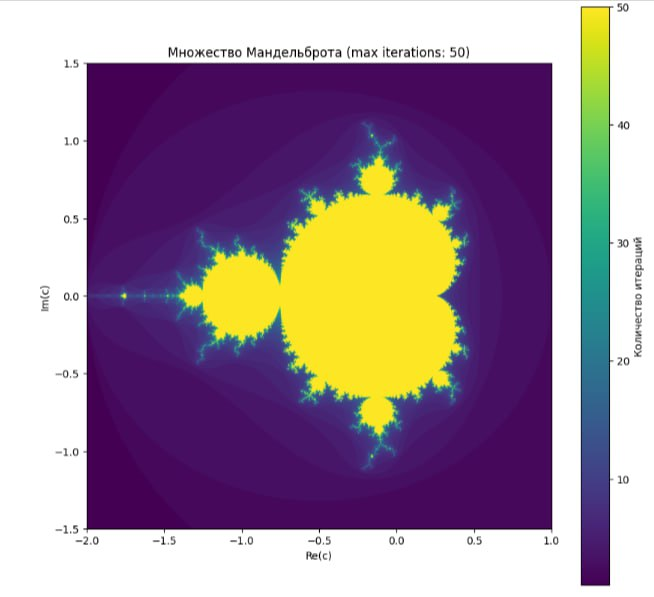
\includegraphics[width=\textwidth]{plots/M1.jpg}
        \caption{Множество Мандельброта, 50~итераций}
    \end{subfigure}
    \hspace{1.7cm}
    \begin{subfigure}{0.4\textwidth}
        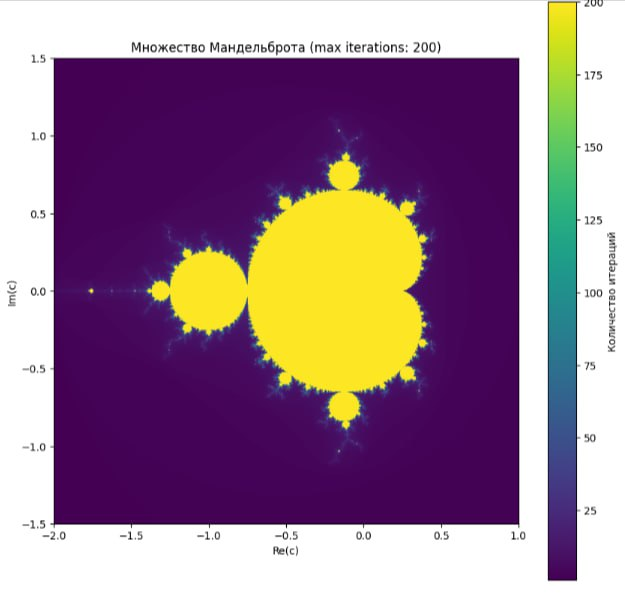
\includegraphics[width=\textwidth]{plots/M2.jpg}
        \caption{Множество Мандельброта, 200~итераций}
    \end{subfigure}
    \\
    \begin{subfigure}{0.4\textwidth}
        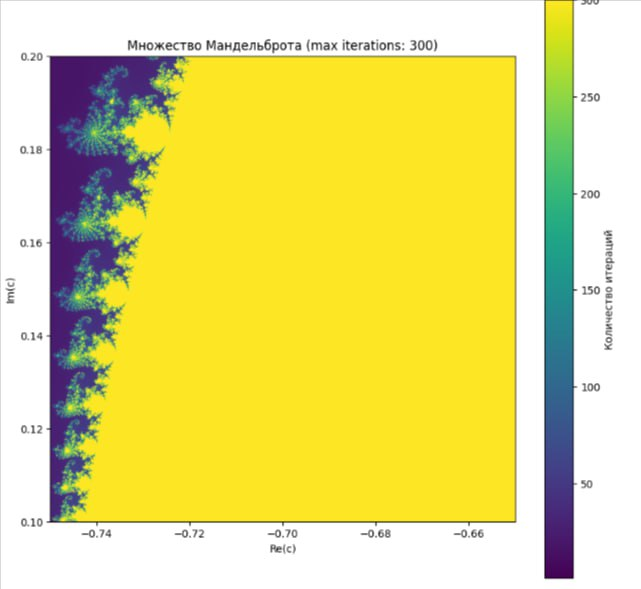
\includegraphics[width=\textwidth]{plots/M3.jpg}
        \caption{Приближение множества Мандельброта, 300 итераций }
    \end{subfigure}
    \hspace{1.7cm}
    \begin{subfigure}{0.4\textwidth}
        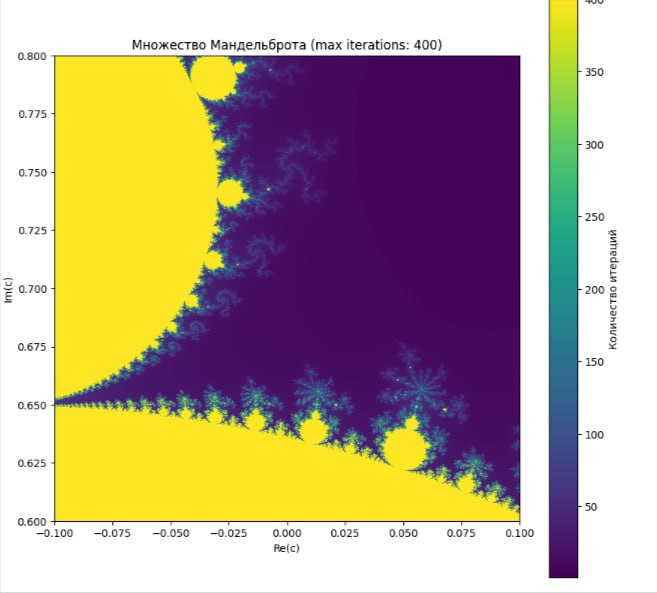
\includegraphics[width=\textwidth]{plots/M4.jpg}
        \caption{Приближение множества Мандельброта на стыке, 400~итераций }
    \end{subfigure}
    \hspace{1.7cm}
    \begin{subfigure}{0.4\textwidth}
        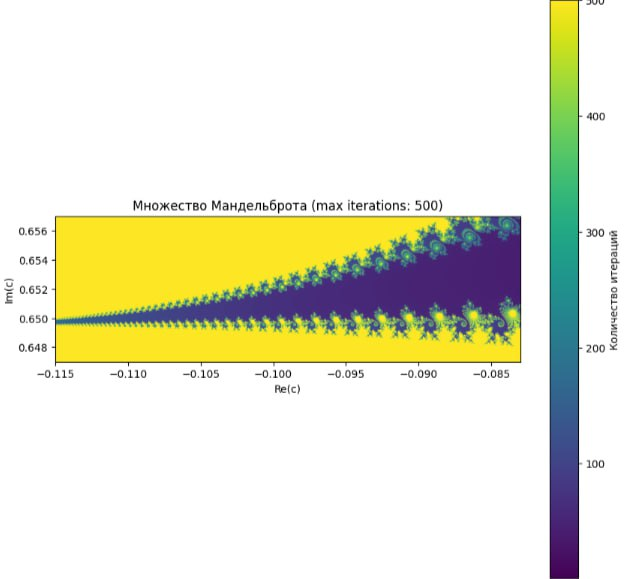
\includegraphics[width=\textwidth]{plots/M5.jpg}
        \caption{Приближение множества Мандельброта по центру слева, 400~итераций }
    \end{subfigure}
    \hspace{1.7cm}
    \begin{subfigure}{0.4\textwidth}
        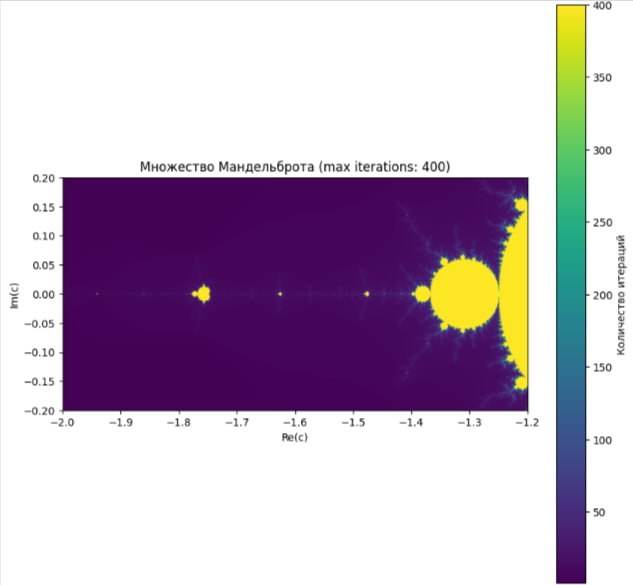
\includegraphics[width=\textwidth]{plots/M6.jpg}
        \caption{Максимальное приближение множества Мандельброта, 500~итераций }
    \end{subfigure}
\end{figure}